\documentclass[a4paper,14pt]{article}
\usepackage[utf8]{inputenc}
\usepackage[T1]{fontenc}
\usepackage[english]{babel}
\usepackage{color}
\usepackage{graphicx}
\pagecolor{white}
\usepackage{lmodern}
\usepackage{amsmath}
\usepackage{amsthm}
\usepackage{amssymb}
\usepackage{mathrsfs}
\usepackage{geometry}
\usepackage{lastpage} 
\usepackage{fancyhdr}
%Define the listing package
\usepackage{listings} %code highlighter
\usepackage{color} %use color
\definecolor{mygreen}{rgb}{0,0.6,0}
\definecolor{mygray}{rgb}{0.5,0.5,0.5}
\definecolor{mymauve}{rgb}{0.58,0,0.82}
 
%Customize a bit the look
\lstset{ %
backgroundcolor=\color{white}, % choose the background color; you must add \usepackage{color} or \usepackage{xcolor}
basicstyle=\footnotesize, % the size of the fonts that are used for the code
breakatwhitespace=false, % sets if automatic breaks should only happen at whitespace
breaklines=true, % sets automatic line breaking
captionpos=b, % sets the caption-position to bottom
commentstyle=\color{mygreen}, % comment style
deletekeywords={...}, % if you want to delete keywords from the given language
escapeinside={\%*}{*)}, % if you want to add LaTeX within your code
extendedchars=true, % lets you use non-ASCII characters; for 8-bits encodings only, does not work with UTF-8
frame=single, % adds a frame around the code
keepspaces=true, % keeps spaces in text, useful for keeping indentation of code (possibly needs columns=flexible)
keywordstyle=\color{blue}, % keyword style
% language=Octave, % the language of the code
morekeywords={*,...}, % if you want to add more keywords to the set
numbers=left, % where to put the line-numbers; possible values are (none, left, right)
numbersep=5pt, % how far the line-numbers are from the code
numberstyle=\tiny\color{mygray}, % the style that is used for the line-numbers
rulecolor=\color{black}, % if not set, the frame-color may be changed on line-breaks within not-black text (e.g. comments (green here))
showspaces=false, % show spaces everywhere adding particular underscores; it overrides 'showstringspaces'
showstringspaces=false, % underline spaces within strings only
showtabs=false, % show tabs within strings adding particular underscores
stepnumber=1, % the step between two line-numbers. If it's 1, each line will be numbered
stringstyle=\color{mymauve}, % string literal style
tabsize=2, % sets default tabsize to 2 spaces
title=\lstname % show the filename of files included with \lstinputlisting; also try caption instead of title
}
%END of listing package%
 
\definecolor{darkgray}{rgb}{.4,.4,.4}
\definecolor{purple}{rgb}{0.65, 0.12, 0.82}
 
%define Javascript language
\lstdefinelanguage{JavaScript}{
keywords={typeof, new, true, false, catch, function, return, null, catch, switch, var, if, in, while, do, else, case, break},
keywordstyle=\color{blue}\bfseries,
ndkeywords={class, export, boolean, throw, implements, import, this},
ndkeywordstyle=\color{darkgray}\bfseries,
identifierstyle=\color{black},
sensitive=false,
comment=[l]{//},
morecomment=[s]{/*}{*/},
commentstyle=\color{purple}\ttfamily,
stringstyle=\color{red}\ttfamily,
morestring=[b]',
morestring=[b]"
}
 
\lstset{
language=JavaScript,
extendedchars=true,
basicstyle=\footnotesize\ttfamily,
showstringspaces=false,
showspaces=false,
numbers=left,
numberstyle=\footnotesize,
numbersep=9pt,
tabsize=2,
breaklines=true,
showtabs=false,
captionpos=b
}
\lhead{Groupe xx}
\rhead{INFO4127}
\cfoot{\date{27 Décembre 2020}}
\rfoot{\thepage/ \pageref{LastPage}}
\renewcommand{\footrulewidth}{0.2mm}
\pagestyle{fancy}
\geometry{hmargin=2.5cm,vmargin=1.5cm}
\graphicspath{ {./images/} }

\newcommand{\horrule}[1]{\noindent\rule{\linewidth}{#1}}

\title{
    \horrule{0.5pt} \\ [0.4cm]
    \Huge Expose Groupe xx INFO 4127 TECHNIQUE D'OPTIMISATION\\ THEME: \\ MÉTHODE DES SUITES DE FIBONACCI\\
    \horrule{2pt} \\[0.5cm]
\begin{center}

\includegraphics[width=100px]{univyde1}\\[15pt]
\end{center}
    \usefont{OT1}{bch}{b}{n}
    \normalfont \normalsize \textsc{Université de Yaoundé I\\University of Yaounde I} \\ [25pt]
    \normalfont \normalsize \textsc{Département D'Informatique\\Department of Computer Science} \\ [20pt]
 }
\author{
    \normalfont                                 
    OUSSAH SIGHA Sony Nelson Matricule 19W2631 \\[5pt]
    FEZEU GHOMSI Eugene Clotaire Matricule 17Q2864 \\[5pt] 
    \normalsize
}
\date{27 Décembre 2020}

\newtheorem*{lemma}{Lemme}
\newtheorem*{définition}{Définition}

\begin{document}

\maketitle

\pagebreak

\addcontentsline{toc}{section}{INTRODUCTION}
\tableofcontents{}

\addcontentsline{toc}{section}{CONCLUSION}

\pagebreak


\section*{INTRODUCTION}

Avant d'entreprendre l'étude de problèmes d'optimisation, il est bon de bien définir ce
qu'est un problème d'optimisation. Dans toute sa généralité, le problème d'optimisation
consiste à déterminer la plus petite (grande) valeur possible qu'une fonction réelle $f$: E $\longrightarrow$ $\mathbb{R}$ nommée fonction objectif puisse prendre dans l'ensemble E nommé ensemble réalisable. Sous forme mathématique, ceci s'exprime (pour le cas de la minimisation)

\begin{center}
$ f^{*}(x) = \inf f(x) x \in E $ .
\end{center}

Il existe plusieurs techniques d'optimisations classifiés selon que certains problèmes a optimiser sont avec ou sans contraintes. Nous étudierons ici une méthode d'optimisation sans contrainte notamment la \textbf{Méthode de suite Fibonacci}.\\

\section{MÉTHODE DE SUITE DE FIBONACCI}

\subsection{Définition}

La méthode de Fibonacci est une technique d'optimisation sans contraintes directe (recherche de la solution sans dériver $f$) appliqué aux fonctions monodimensionnelle strictement convexe. en d'autre terme elle s'applique sur des fonctions a une variable  . L'approche de Fibonacci est une variante plus optimal de la méthode de dichotomie étant donnée que le choix du nouvel intervalle $[a^{k}; b^{k}]$ se fait suivant les nombres issue de la suite de Fibonacci, elle est aussi très adapté lorsque trouver la dérivée de la fonction à optimiser s'avère difficile.

\subsection{Condition d'utilisation}

Une méthode de recherche directe est une méthode qui repose uniquement sur l'évaluation de $f(x)$ sur une
séquence $x_{1}, x_{2},..., x_{n}$ et comparer des valeurs afin de trouver un optimiseur de $f$.
Les méthodes directes sont généralement appliquées dans les circonstances suivantes:
\begin{itemize} 
	\item la fonction $f(x)$ n'est pas différentiable;
    \item les dérivées de $f$ sont compliquées à calculer ou même inexistantes;
    \item la fonction a peu de variables;
    \item l'emplacement d'une solution optimale est à peu près connu.   
\end{itemize}.

\subsection{Principe}

De façon générale le principe de la méthode de suite de Fibonacci est basé sur le lemme suivant:

\begin{lemma}
Soit $f$: [a;b] $\longrightarrow$ $\mathbb{R}$ une fonction uni-modale et $x^{D}$, $x^{G}$ tels que a < $x^{G}$ < $x^{D}$ < b alors:

\begin{list}{•}{ }
\item$f(x^{G}) < f(x^{D}) \Longrightarrow \widehat{x} \in [a; x^{D}]$
\item$f(x^{G}) > f(x^{D}) \Longrightarrow \widehat{x} \in [x^{G}; b]$
\item$f(x^{G}) = f(x^{D}) \Longrightarrow \widehat{x} \in [x^{G}; x^{D}]$, $\widehat{x}$ représente l'optimum (minimum ou maximum) rechercher.
\end{list}

\end{lemma}

La spécificité de cette méthode réside dans le choix des points $x^{G}$ et $x^{D}$. En effet ces points sont déterminés par les nombre de la suite de Fibonacci. Pour rappel la suite de Fibonacci se définit comme suit:
	\[F_{0} = F_{1} = 1\]
	\[F_{k+2} = F_{k+1} + F_{k}\]
	\[\lim_{k\rightarrow\infty} \frac{F_{k+1}}{F_{k}} \longrightarrow \frac{1+\sqrt{5}}{2}\]
les point $x^{G}$ et $x^{D}$ sont donc définis de manière suivante: 
\[
	x^{G}_{k} = a_{k} + \frac{F_{N-k}}{F_{N+2-k}}(b_{k} - a_{k}), x^{D}_{k} = a_{k} + \frac{F_{N+1-k}}{F_{N+2-k}}(b_{k} - a_{k})
\]

on utilise ensuite le lemme précédent pour trouver l'intervalle dans lequel le minimum peut se trouver et on s'arrête après un nombre N d'itérations.

\subsection{Performance et Limites}

Étant donnée que les nombres de la suite de Fibonacci croissent rapidement vers l'infini, les distances des intervalles $[a_{k}; b_{k}]$ tendent plus rapidement vers 0 ce qui fait de la méthode des suites de Fibonacci la méthode qui converge plus rapidement que toutes autre méthode d'optimisation sans contraintes mono-linéaire.
La méthode des suites de Fibonacci requiert un nombre N d'itérations, ainsi lorsque N $\longrightarrow$ $\infty$ la complexité de l'algorithme s'en trouve lourdement impacté. La méthode de section dorée vient donc compléter celle des suites de Fibonacci en se basant sur le fait que \[\lim_{N\rightarrow\infty} \frac{F_{N+1}}{F_{N}} \longrightarrow \frac{1+\sqrt{5}}{2}\] en posant donc $\tau = \frac{1+\sqrt{5}}{2}$ (Le nombre d'or, d’où le nom de \textbf{section dorée}) on peut écrire \[\lim_{N\rightarrow\infty} \frac{F_{N}}{F_{N+1}} \longrightarrow \frac{1}{\tau}\]. Et donc les points $x^{G}$ et $x^{D}$ peuvent se réécrire indépendamment de N comme suit:

\[
	x^{G}_{k} = a_{k} + \frac{1}{\tau}(b_{k} - a_{k}), x^{D}_{k} = a_{k} + \frac{1}{\tau}(b_{k} - a_{k})
\]

\subsection{Algorithme}

Lorsqu'on connaît le principe de la méthode , l'algorithme de Fibonacci se déduit facilement.

\subsubsection{Simulateur ou évaluation de la fonction aux point ak et bk}

\begin{list}{•}{ }

\item on se donne N = nombre total de fois ou l'on évaluera $f$ en un point
\item initialisation : $a_{1} = a, b_{1} = b$
\item itérations : \[x_{k}^{G} = a_{k} + \frac{F_{N-k}}{F_{N+2-k}}(b_{k} - a_{k})\]  et \[x_{k}^{D} = a_{k} + \frac{F_{N+1-k}}{F_{N+2-k}}(b_{k}-a_{k})\]
\item Si:
\begin{itemize}
\item[-] $f(x_{k}^{G}) < f(x_{k}^{D}) \Longrightarrow a_{k+1} = a_{k} et b_{k+1} = x_{k}^{D}$
\item[-] $f(x_{k}^{G}) > f(x_{k}^{D}) \Longrightarrow a_{k+1} = x_{k}^{G} et b_{k+1} = b_{k}$
\item[-] $f(x_{k}^{G}) = f(x_{k}^{D}) \Longrightarrow a_{k+2} = x_{k}^{G} et b_{k+2} = x_{k}^{D}$
\end{itemize}

\item arrêt : après N itérations.
    
\end{list}

\subsubsection{Optimiseur ou choix des points ak+1 et bk+1}

Calcul de $x_{k+1}^{D}$ et $x_{k+1}^{G}$ :\\
\begin{itemize}
\item[$\blacktriangleright$] cas $f (x_{k}^{G}) < f (x_{k}^{D})$
\end{itemize}
\begin{list}{•}{}
	\item $a_{k+1} = a_{k}$ et $b_{k+1} = x_{k}^{D}$
	\item $x_{k+1}^{D} = a_{k+1} + \frac{F_{N+1-(k+1)}}{F_{N+2-(k+1)}}(b_{k+1}-a_{k+1})$
	\item $= a_{k} + \frac{F_{N-k}}{F_{N+1-k}}(x_{k}^{D} - a_{k})$
	\item $= a_{k} + \frac{F_{N-k}}{F_{N+1-k}} \times \frac{F_{N+1-k}}{F_{N+2-k}}(b_{k}-a_{k})$
	\item $= a_{k} + \frac{F_{N-k}}{F_{N+2-k}}(b_{k}-a_{k})$
	\item $= x_{k}^{G}$
\end{list}
Donc seul $f(x_{k+1}^{G})$ doit être évaluer à l'itération k+1.
Longueur de l'intervalle : $b_{k+1}-a_{k+1} = x_{k}^{D}-a_{k} = \frac{F_{N+1-k}}{F_{N+2-k}}(b_{k}-a_{k})$.\\
\begin{itemize}
\item[$\blacktriangleright$] Cas $f (x_{k}^{G}) > f (x_{k}^{D})$
\end{itemize}
Ce déduit du cas précédent par symétrie. Seul $f(x_{k+1}^{D})$ doit être évaluer à l'itération k+1, et
longueur de l'intervalle : $b_{k+1}-a_{k+1} = x_{k}^{D}-a_{k} = \frac{F_{N+1-k}}{F_{N+2-k}}(b_{k}-a_{k})$.\\
\begin{itemize}
\item[$\blacktriangleright$] Cas $f (x_{k}^{G}) = f (x_{k}^{D})$
\end{itemize}
$f(x_{k+2}^{G})$ et $f(x_{k+2}^{D})$ doivent être évalués
$b_{k+2}-a{k+2} \leq \frac{F_{N-k}}{F_{N+2-k}}(b_{k}-a_{k})$.\\

A la sortie de l'algorithme la longueur de l'intervalle 
\[
(b_{N}-a_{N}) \leq \prod_{k=1}^{N-1}\frac{F_{N+1-k}}{F_{N+2-k}}(b-a) = \frac{(b-a)}{F_{N+1}} 
\]

\section{CHOIX DES FONCTION POUR L’IMPLÉMENTATION DE LA MÉTHODE DES SUITES DE FIBONACCI}

Les fonction uni-modales choisies pour l’application de la méthode des suites de Fibonacci sont les suivantes:

$f(x) = \exp^{x(x-1)}$ sur $[-1;1]$ et $g(x) = x^{2}(1-\cos(x))$ sur $[-1;\frac{1}{2}]$.

\subsection{Vérification de L'hypothèse d'Uni-modalité}
\begin{définition}
	Une fonction $f$, partout définie sur I, est dite \textbf{uni-modale} sur I si :
	\begin{list}{•}{}
	\item elle admet un unique minimum $\widehat{x}$ dans I
	\item elle est strictement décroissante sur I $\cap$ $]-\infty;\widehat{x}[$ et strictement croissante sur I $\cap$ $]\widehat{x}, +\infty[$\\
	\end{list}
\end{définition}

\begin{itemize}
\item[$\blacktriangleright$] Pour la fonction $f(x) = \exp^{x(x-1)}$ sur $[-1;1]$ on a:
\end{itemize}

\[ f'(x)=0 \Leftrightarrow (2x-1)\exp^{x(x-1)} = 0 \] L'unique solution est $\frac{1}{2}$ $\in$ $[-1;1]$. La première condition est donc vérifier. De plus $f'(x)$ est strictement décroissante sur $[-1;\frac{1}{2}[$ $=$ $[-1;1]$ $\cap$ $]-\infty;\frac{1}{2}[$ et strictement croissante sur $]\frac{1}{2};1]$ $=$ $[-1;1]$ $\cap$ $]\frac{1}{2}, +\infty[$, ainsi les deux propriétés sont vérifiées. Donc $f(x) = \exp^{x(x-1)}$ sur $[-1;1]$ est uni-modale.\\

\begin{itemize}
\item[$\blacktriangleright$] Pour la fonction $g(x) = x^{2}(1-\cos(x)) sur [-1;\frac{1}{2}]$ on a:
\end{itemize}

\[ g'(x)=0 \Leftrightarrow 2x(1-\cos(x)) + x^{2}\sin(x) = 0 \] L'unique solution est $0 \in [-1;\frac{1}{2}]$. La première condition est donc vérifier. De plus $g'(x)$ est strictement décroissant sur $[-1;0[ = [-1;\frac{1}{2}] \cap ]-\infty;0[$ et strictement croissante sur $]0;\frac{1}{2}] = [-1;\frac{1}{2}] \cap ]\frac{1}{2}, +\infty[$, ainsi les deux propriétés sont vérifiées. Donc $g(x) = x^{2}(1-\cos(x)) sur [-1;\frac{1}{2}]$ est uni-modale.

\section{IMPLÉMENTATION DE LA MÉTHODE DES SUITES DE FIBONACCI}

\subsection{Présentation du Code source}

L’implémentation (code en javascript) de l'algorithme de Fibonacci est la suivante \\

\begin{lstlisting}[language=JavaScript]
function fib(n) {
	const preCalculated = Array(n + 1).fill(0)
	preCalculated[1] = 1

	for (var i = 0; i <= n; i++) {
		preCalculated[i + 2] = preCalculated[i + 1] + preCalculated[i]
	}

	return preCalculated[n]

}
\end{lstlisting}

La génération de valeur de fait lors de la phase d'initialisation et celle d'itération.

\begin{lstlisting}[language=JavaScript]
    function FIBSearch(f,a,b,T){
      var L, M, j, C, x1, x2, N, val;
      L = (b-a)/T;
      M = Math.round(L);
      j=0;
      do{
        C = fib(j);
        if( C<L ){
          j = j+1;
          
        }
      }while(C<L);
      N = j;
      x1 = a+(fib(N-2)/fib(N))*(b-a);
      x2 = a+(fib(N-1)/fib(N))*(b-a);
      iterate(f,a,b,N,x1,x2);
    }
        function iterate(f,a,b, N,x1,x2){
      var x1n = [],x2n = [],an = [],bn = [],i,fx1=[],fx2 = [],j,fmid;

      
     i = 1;
     x1n[1] = x1;
     x2n[1] = x2;
     an[1] = a;
     bn[1] = b;
     i = 1;

    for(var j=1; j < N + 1; j++){
      
      fx1[i] = evalf(f,x1n[i]);
      fx2[i] = evalf(f,x2n[i]);
      if (fx1[i]<=fx2[i]){
        an[i+1] = x1n[i];
        bn[i+1] = bn[i];
        x1n[i+1] = x2n[i];
        x2n[i+1] = an[i+1]+(fib(N-i-1)/fib(N-i))*(bn[i+1]-an[i+1]);

      }else{
        an[i+1] = an[i];
        bn[i+1] = x2n[i];
        x2n[i+1] = x1n[i];
        x1n[i+1] = an[i+1]+(fib(N-i-2)/fib(N-i))*(bn[i+1]-an[i+1]);
        
      }
      i = i+1;
        
        mdpt = (an[i] + bn[i])/2;
        if((i+2)==N){
          if(evalf(f, an[i]) > evalf(f,bn[i]) || evalf(f, an[i]) > evalf(f,mdpt)){
            fkeep = evalf(f,an[i]); 
            xkeep = an[i];
          }else{
            if(evalf(f,bn[i]) > evalf(f,mdpt)){
              fkeep = evalf(f,bn[i]); 
              xkeep = evalf(f,bn[i]);
            }else{
              fkeep =  evalf(f,mdpt); 
              xkeep = mdpt;
            } 
          }
        }
    }
   
    
  }
    
\end{lstlisting}

Le code qui nous intéresse ici est:
\begin{lstlisting}[language=JavaScript]   
      x1 = a+(fib(N-2)/fib(N))*(b-a);
      x2 = a+(fib(N-1)/fib(N))*(b-a);
\end{lstlisting}

On génère ainsi les x a tester. lors de la phase d'itération les x sont généré a partir des nouvelles bornes de l'intervalle 
\begin{lstlisting}[language=JavaScript]   
        x1n[i+1] = x2n[i];
        x2n[i+1] = an[i+1]+(fib(N-i-1)/fib(N-i))*(bn[i+1]-an[i+1]);
\end{lstlisting}

\begin{lstlisting}[language=JavaScript]   
        x2n[i+1] = x1n[i];
        x1n[i+1] = an[i+1]+(fib(N-i-2)/fib(N-i))*(bn[i+1]-an[i+1]);
\end{lstlisting}

Ces deux portions de code permettent donc de générer les valeurs a tester. l'optimiseur est constituer d'une condition qui nous permet de réduire l'intervalle de valeur a chaque itération.
  
\begin{lstlisting}[language=JavaScript]   
        if (fx1[i]<=fx2[i])
\end{lstlisting}

\subsection{Presentation du logiciel}
\begin{figure}[h]
\centering
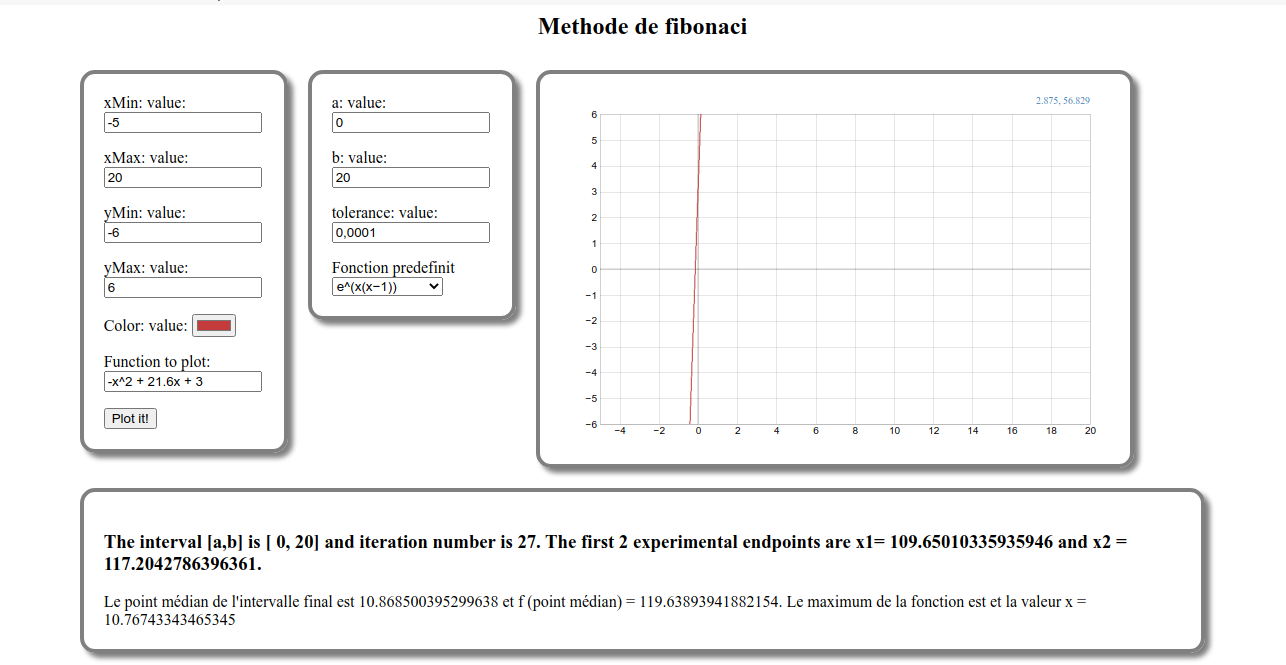
\includegraphics[width=1\textwidth, scale=1.1]{c}
\caption{Interface du logiciel}
\label{fig:figure1}
\end{figure}

L'interface du logiciel est assez intuitif. En effet sur l'image précédente le processus d'utilisation peut être décris avec les étapes suivantes:

\begin{list}{•}{}
\item Choisir les valeurs maximum et minimums des axe des abscisses et des ordonnées pour le tracé de la fonction
\item Entrer le nombre d'itérations
\item Choisir l'intervalle de recherche de solution
\item Écrire la fonction a tracer et valider
\end{list}

Les résultats de la méthode de Fibonacci s'afficheront dans le block en bas du trace de la fonction.

\pagebreak

\section*{CONCLUSION}
La méthode de Fibonacci est une technique d'optimisation sans contraintes directe appliqué au fonction uni-modale. dû au fait que le découpage de l'intervalle en sous intervalle pour rechercher la solution dépend des nombres de la suite de Fibonacci cette méthode converge très rapidement vers la solution et fait d'elle la méthode la plus efficace partie les technique de son genre, néanmoins un inconvénient de cette méthode est qu'il faut fixer au préalable un nombre \textbf{N} d'itération donc si \textbf{N} est mal fixé (N trop petit) on pourrait en ressortir avec une solution qui n'est pas optimale. Pour palier a ce problème une autre méthode dite de section dorée base sur celle de Fibonacci a été mise au point. La méthode de Fibonacci a un principe des plus simple et son algorithme est assez simple a implémenter, ceci fait de cette méthode une technique assez peu pratique devant des problèmes réels de l'informatique qui ont parfois beaucoup de contraintes et plusieurs solutions optimales. 

\end{document}
